\section{LARS}
LARS algoritmen blev introduceret i \citep{efron}. 
Først vil vi beskrive LARS algoritmen, hvorefter vi vil introducere en simpel modifikation, som fører til lasso estimater. \\[2mm]
%
I grove træk fungerer algoritmen som følgende. 
Først sættes alle koefficienter lig nul, og vi finder prædiktoren som er mest korreleret med responsvariablen \(\y\), denne prædiktor betegnes \(x_{j_1}\).
Der udføres en simpel lineær regression af \(\y\) på \(x_{j_1}\), hvoraf vi finder en residualvektor.
%som herefter betragtes som responsvariablen.
Herefter tages det størst mulige step i retningen af denne prædiktor indtil en anden prædiktor, som betegnes \(x_{j_2}\), har samme korrelation med den nuværende residual.
Istedet for at fortsætte langs \(x_{j_1}\), fortsætter LARS i en retning som er ensvinklet mellem de to prædiktorer indtil en tredje variabel bliver den mest korreleret mængde.
LARS fortsætter da ensvinklet imellem \(x_{j_1}\), \(x_{j_2}\) og \(x_{j_3}\), dvs langs ``least angle direction'' indtil en fjerde variable medtages, osv.

LARS finder estimaterne \(\widehat{\tmu} = \X \widehat{\tbeta}\), ved at tilføjes én prædiktor i hvert step til modellen, således at efter \(k\) steps er præcis \(k\) af disse \(\hat{\beta}_j\) forskellig fra nul.

Figur \ref{fig:lars} illustrerer algoritmen, hvor $p = 2$ og $\X = \del{\textbf{x}_1, \textbf{x}_2}$.
I dette tilfælde afhænger de nuværende korrelationer, givet ved \(\textbf{c}\del{\boldsymbol{\widehat{\mu}}} = \X^T\del{\textbf{y} - \widehat{\boldsymbol{\mu}}}\), kun af projektionen \(\bar{\y}_2\) af \(\y\) på det lineære rum $\mathcal{L} \del{\X}$ udspændt af \(\x_1\) og \(\x_2\), dvs 
\begin{align*}
\textbf{c}\del{\boldsymbol{\widehat{\mu}}} =  \X^T \del{ \bar{\y}_2 - \boldsymbol{\widehat{\mu}}}.
\end{align*}
Algoritmen starter i $\widehat{\boldsymbol{\mu}}_0 = \textbf{0}$.
På figur \ref{fig:lars} ses, at \(\bar{\y}_2 - \widehat{\boldsymbol{\mu}}_0\) har en mindre vinkel med \(\x_1\) end \(\x_2\), dvs \(c_1 \del{\widehat{\boldsymbol{\mu}}_0} > c_2 \del{\widehat{\boldsymbol{\mu}}_0}\).
LARS tilføjer derfor \(\widehat{\boldsymbol{\mu}}_0\) i retningen af \(\x_1\), og vi får
\begin{align*}
\widehat{\tmu}_1 = \widehat{\tmu}_0 + \widehat{\gamma}_1 \x_1,
\end{align*}
hvor \(\widehat{\gamma}_1\), som er stepstørrelsen, vælges således at  \(\bar{\y}_2 - \widehat{\tmu}_1\) er ligeså korreleret med \(\x_1\) som med \(\x_2\).
Dermed halverer \(\bar{\y}_2 - \widehat{\boldsymbol{\mu}}_1\) vinklen mellem \(\x_1\) og \(\x_2\) således at \(c_1 \del{\widehat{\boldsymbol{\mu}}_1} = c_2 \del{\widehat{\boldsymbol{\mu}}_1}\).
%
\begin{figure}[H]
\centering
\scalebox{0.8}{\begin{tikzpicture}
%\draw [<-] (4,0) node [below] {$\x_1$}-- (-3,0);
\draw [blue] [<-] (1,0) node [below] {$\widehat{\tmu}_1$} -- (-3,0);
\draw [<-] (4,0) node [below] {$\x_1$} -- (1,0);
\filldraw [blue] (1,0) circle (2pt) node [below, black] {$\widehat{\boldsymbol{\mu}}_1$};
\filldraw [green] (-3,0)  circle (2pt) node [below, black]{$\widehat{\boldsymbol{\mu}}_0$};
\draw [dashed] [<-] (5,4) node [above] {$\x_2$} --(1,0);
\draw [<-] (1,4) node [above] {$\x_2$} --(-3,0);

\draw [green] (5,1.66) node [above, black] {$\bar{\y}_2$} -- (-3,0);
\filldraw [green] (5,1.66) circle (2pt);
\draw [blue] [->] (1,0) -- (3, 0.83) node [below, black] {$\mathbf{u}_2$} ;
\draw [green] (3,0.83) -- (5,1.66) ; 

\draw [green] (5,0) node [below] {} -- (4.1,0);
\filldraw [green] (5,0) circle (2pt) ;
\draw (5,0) node [black, below] {$\bar{\y}_1$};
\end{tikzpicture}}
\caption{LARS algoritmen for \(p=2\). \(\bar{\y}_2\) er projektionen af \(\y\) på det lineære underrum \(\mathcal{L} \del{\x_1, \x_2}\).
Med start i \(\widehat{\tmu}_0=\mathbf{0}\), har residualvektoren \(\bar{\y}_2 - \widehat{\tmu}_0\) en større korrelation med \(\x_1\) end \(\x_2\). Næste LARS estimat er \(\widehat{\tmu}_1 = \widehat{\tmu}_0 + \widehat{\gamma}_1 \x_1\), hvor \(\widehat{\gamma}_1\) vælges således at \(\bar{\y}_2 - \widehat{\tmu}_1\) halverer vinklen mellem \(\x_1\) og \(\x_2\). Da er \(\widehat{\tmu}_2 = \widehat{\tmu}_1 + \widehat{\gamma}_2 \mathbf{u}_2\), hvor \(\mathbf{u}_2\) er en enhedsvektor som ligger langs denne halveringslinje.
Der gælder at \(\widehat{\tmu}_2 = \bar{\y}_2\) for \(p=2\), dette er ikke tilfældet for \(p>2\), som ses på figur \ref{fig:lars2}.
 }\label{fig:lars}
\end{figure}
%
Lad $\mathbf{u}_2$ være enhedsvektoren, som ligger langs denne halveringslinje.
Det næste LARS estimat er dermed
\begin{align*}
\widehat{\boldsymbol{\mu}}_2 = \widehat{\boldsymbol{\mu}}_1+ \widehat{\gamma}_2 \mathbf{u}_2,
\end{align*}
hvor $\widehat{\gamma}_2$ vælges således at $\widehat{\boldsymbol{\mu}}_2 = \bar{\textbf{y}}_2$ i tilfældet hvor $p = 2$. 
For \(p>2\), da vil stepstørrelsen \(\widehat{\gamma}_2\) være mindre, hvilket fører til en anden ændring af retningen, som illustreres på figur \ref{fig:lars2}.
%
\begin{figure}[H]
\centering
\scalebox{0.8}{\begin{tikzpicture}
\filldraw [green] (-3,0) circle (2pt) node [below, black]{$\widehat{\tmu}_0$};
\draw [<-] (6.8,0) node [below] {$\x_1$} -- (-3,0);
\draw [<-] (1,4) node [above] {$\x_2$} --(-3,0);
\draw [<-] (-5,4) node [above] {$\x_3$} --(-3,0);

\draw [green] (4,0) node [above, black] {$\bar{\y}_1$} -- (-3,0);
\filldraw [green] (4,0) circle (2pt) ;
\draw [blue] (1,0) node [below, black] {$\widehat{\tmu}_1$} -- (-3,0);
\draw [blue] [->] (-3,0) -- (-1.5, 0) node [below, black] {$\mathbf{u}_1$} ;

\draw [green] (6,2.1) node [above, black] {$\bar{\y}_2$} -- (1,0);
\filldraw [green] (6,2.1) circle (2pt) ;
\draw [blue] (4,1.25) node [below, black] {$\widehat{\tmu}_2$} -- (1,0);
\draw [blue] [->] (1,0) -- (2.6, 0.65) node [below, black] {$\mathbf{u}_2$} ;

\draw [green] (5,3.5) node [above, black] {$\bar{\y}_3$} -- (4,1.25);
\filldraw [green] (5,3.5) circle (2pt) ;
\draw [blue] [<-] (4.4,2.2)  -- (4,1.25);
\draw [blue] (4.8,3.1)-- (4.4,2.2);
\draw [blue] [<-] (4.5,3.5) -- (4.8,3.1);
\end{tikzpicture}}
\caption{I hvert step nærmer LARS estimatet \(\hat{\tmu}_k\) sig det tilhørende OLS estimat \(\bar{\y}_k\), men vil aldrig nå det.
 }\label{fig:lars2}
\end{figure}
%
Vi antager, at prædiktorerne \(\x_1, \ldots, \x_p\) er lineært uafhængige.
Lad \(\A\) være en delmængde af indekser \(\cbr{1,\ldots, p}\), og definer matricen
\begin{align}
\X_\A = \del{\dots s_j \x_j \dots}_{j \in \A}, \label{eq:lars_2.4}
\end{align}
hvor  $s_j = \pm 1$, således at \(\X_\A\) er en matrix bestående af kolonnerne af \(\X\) som er inkluderet i \(\mathcal{A}\) multipliceret \(s_j\).
Lad 
\begin{align}
N_\A = \X_\A^T \X_\A \quad \text{og} \quad A_\A = \del{\mathbf{1}_\A^T N_\A^{-1} \mathbf{1}_\A}^{-1/2}, \label{eq:lars_2.5}
\end{align}
hvor \(\mathbf{1}_\A\) er en vektor bestående af 1-tallet med længde lig antal elementer i \(\A\).
Da defineres en ensvinklet vektor
\begin{align}
\mathbf{u}_\A = \X_\A \omega_\A, \quad \text{hvor } \omega_\A = A_\A N_\A^{-1} \mathbf{1}_\A, \label{eq:lars_2.6}
\end{align}
som er en enhedsvektor, der giver lige vinkler, mindre end \(90^0\), med kolonnerne af \(\X_\A\), dvs
\begin{align}
\X_\A^T \mathbf{u}_\A = A_\A \mathbf{1}_\A \quad \text{og} \quad \Vert \mathbf{u}_\A \Vert^2 = 1. \label{eq:lars_2.7}
\end{align}
Herefter kan vi give en fyldestgørende beskrivelse af LARS algoritmen.
%
\begin{alg} [LARS algoritmen]
\begin{enumerate}
\item Standardisere prædiktorerne og centre responsvariablen. 
Start med \(\widehat{\boldsymbol{\mu}}_0 = \mathbf{0}\), \(\widehat{\mathbf{c}} = \X^T \y\), og \(\A = \emptyset\).
\item Find prædiktoren \(\tx_j\) som er mest korreleret med ???? y og noegt residual!!! og definer den aktive mængde \(\A = \cbr{j}\).
\item Gentag følgende indtil alle prædiktorer fra \(\A^C\) er i den aktive mængde:
\begin{itemize}
\item Antag \(\widehat{\boldsymbol{\mu}}_\A\) er det nuværende LARS estimat og at
\begin{align}
\widehat{\mathbf{c}} = \X^T \del{\y - \widehat{\boldsymbol{\mu}}_\A}, \label{eq:lars_2.8}
\end{align} 
er vektoren af nuværende korrelationer.
Den aktive mængde \(\A\) er en mængde af indekser svarende til prædiktorer med størst absolut nuværende korrelationer
\begin{align}
\widehat{C} = \max_j \cbr{\abs{\widehat{c}_j}} \quad \text{og} \quad \A= \cbr{j: \ \abs{ \widehat{c}_j} = \widehat{C}}. \label{eq:lars_2.9}
\end{align}
Lad 
\begin{align*}
s_j = \text{sign} \cbr{\widehat{c}_j}, \quad j \in \A,
\end{align*}
da udregnes \(\X_\A\), \(A_\A\) og \(\mathbf{u}_\A\) som i \eqref{eq:lars_2.4}-\eqref{eq:lars_2.6}  samt vektoren af indre produkt
\begin{align*}
\mathbf{a} = \X^T \mathbf{u}_\A.
\end{align*}
\item Opdatere \(\widehat{\boldsymbol{\mu}}_\A\) til
\begin{align}
\widehat{\boldsymbol{\mu}}_{\A_+} = \widehat{\boldsymbol{\mu}}_\A + \widehat{\gamma} \mathbf{u}_\A, \label{eq:lars_2.12}
\end{align}
hvor 
\begin{align}
\widehat{\gamma} = \min_{j \in \A^c}^+ \cbr{ \frac{\widehat{C}- \widehat{c}_j}{A_\A - a_j} , \frac{\widehat{C} + \widehat{c}_j}{A_\A + a_j}}, \label{eq:lars_2.13}
\end{align}
og hvor \(\min^+\) indikerer at minimum kun tages over de positive komponenter indenfor valget af \(j\) i \eqref{eq:lars_2.13}.
\item Sæt \(\A = \A \cup \cbr{\hat{j}}\), hvor \(\hat{j}\) er minimeringsindekset i \eqref{eq:lars_2.13}.
\end{itemize}
\end{enumerate}
\end{alg}
%
Formlerne \eqref{eq:lars_2.12} og \eqref{eq:lars_2.13} har følgende fortolkning.
Definer
\begin{align}
\tmu \del{\gamma} = \widehat{\tmu}_\A + \gamma \mathbf{u}_\A, \label{eq:lars_2.14}
\end{align}
for \(\gamma > 0\), således at den nuværende korrelation er givet ved
\begin{align}
c_j \del{\gamma} = \x_j^T \del{\y - \tmu \del{\gamma}} = \widehat{c}_j - \gamma a_j. \label{eq:lars_2.15}
\end{align}
For \(j \in \A\) giver \eqref{eq:lars_2.7}-\eqref{eq:lars_2.9} at
\begin{align}
\abs{c_j \del{\gamma}} = \widehat{C} - \gamma A_\A,\label{eq:lars_2.16}
\end{align}
som viser, at alle af de maksimale absolutte nuværende korrelationer falder ligeligt.
For \(j \in \A^C\), viser \eqref{eq:lars_2.15} og \eqref{eq:lars_2.16} at \(c_j \del{\gamma}\) er lig den maksimale værdi i \(\gamma = \frac{\widehat{C} - \widehat{c}_j}{A_\A - a_j}\).
Derfor er \(\hat{\gamma}\) i \eqref{eq:lars_2.13} den mindst positive værdi af \(\gamma\) således at et nyt indeks \(\widehat{j}\) tilføjes til den aktive mængde.
\(\hat{j}\) er minimeringsindekset i \eqref{eq:lars_2.13} og den nye aktive mængde \(\A_+\) er \(\A \cup \cbr{\widehat{j}}\) og den nye maksimum absolut korrelation er \(\widehat{C}_+ = \widehat{C}- \widehat{\gamma} A_\A\).
%
\begin{figure}[H]
\centering
\scalebox{0.6}{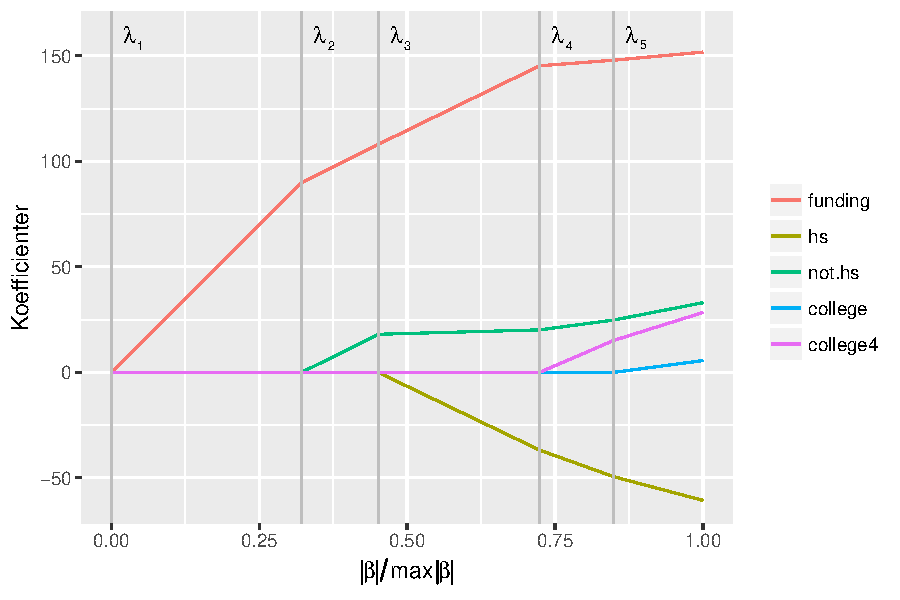
\includegraphics{fig/img/crime_lars_lasso.pdf}}
\caption{Koefficientstierne udregnet med LARS imod fraktion af \(\ell_1\) norm for crime data.} \label{fig:crime_lar}
\end{figure}
%
Figur \ref{fig:crime_lar} illustrerer lars estimaterne som funktion af shrinkage for crime data.
Af figuren kan vi aflæse rækkefølgen, hvori variablerne medtages i modellen.
For \(s=0\), er der ingen variable i modellen, som ses til ventre.
Hvis vi bevæger os mod højre ses at den første variabel som medtages i modellen er variabel 1 (\texttt{funding}), efterfulgt at variabel 3 (\texttt{not.hs}), derefter 2 (\texttt{hs}), variabel 5 (\texttt{college4}) og til slut variabel 4 (\texttt{college}). 
Algoritmen kræver \(p=5\) steps.
%
%Højre figur viser de absolutte nuværende korrelationer
%\begin{align*}
%\abs{\widehat{c}_{kj}} = \abs{\x_j^T \del{\y - \widehat{\tmu}_{k-1}}},
%\end{align*}
%for \(j = 1, \ldots, 5\) som en funktion af LARS step \(k\).
%Den maksimale korrelation
%\begin{align*}
%\widehat{C}_k = \max \cbr{\abs{\widehat{c}_{kj}}} = \widehat{C}_{k-1} - \widehat{\gamma}_{k-1} A_{k-1},
%\end{align*}
%aftager med \(k\) som forventet.
%I hvert step tilføjes en ny variabel \(j\) til den aktive mængde, derfor har vi, at \(\abs{\widehat{c}_{kj}} = \widehat{C}_k\).
%Fortegnet \(s_j\) af hver \(\x_j\) i \eqref{eq:lars_2.4} forbliver konstant, da den aktive mængde kun stiger.

For LARS algoritmen kræves blot \(p\) steps for at finde den fulde løsning.
De beregnings omkostninger for LARS algoritmen er af samme orden, som hvad der kræves for løsningen af mindste kvadraters metode med \(p\) prædiktorer.


\subsection{Lasso modifikation} \label{subsec:lasso_modifikation}
I dette afsnit beskrives en simpel modifikation af LARS algoritmen, således at den giver lasso estimater.
Lad \(\widehat{\tbeta}^\text{lasso}\) være løsningen til lasso problemet \eqref{eq:2.5} med \(\widehat{\tmu}^\text{lasso} = \X \widehat{\tbeta}^\text{lasso}\).
Da kan det vises, at fortegnet af enhver ikke-nul koefficient \(\widehat{\beta}_j\) og fortegnet \(s_j\) af den nuværende korrelation \(\widehat{c}_j = \x_j^T \del{\y - \widehat{\tmu}}\) må stemmes overens
\begin{align}
\text{sign} \del{\widehat{\beta}_j } = \text{sign} \del{\widehat{c}_j } = s_j, \quad j \in \A. \label{eq:lars_3.1}
\end{align}
%
%\begin{lem}
%For \(\widehat{\beta}^\text{lasso}\) må der gælder, at
%\begin{align*}
%\widehat{c}_j = \widehat{C} \cdot \text{sign} \del{\widehat{\beta}_j},
%\end{align*}
%hvor \(\widehat{c}_j = \x_j^T \del{\y - \widehat{\tmu}}= \x_j^T \del{\y - \X \widehat{\beta}}\).
%Dette medfører, at
%\begin{align}
%\text{sign} \del{\widehat{\beta}_j } = \text{sign} \del{\widehat{c}_j }, \quad j \in \A \label{eq:lars_5.29}
%\end{align}
%\end{lem}
%
Denne restriktion er ikke inkluderet i LARS algoritmen, men kan nemt modificeret hertil. 
Antag vi netop har fuldendt et LARS step, som har givet en ny aktive mængde \(\A\) som i \eqref{eq:lars_2.9}, og at det tilhørende LARS estimat \(\widehat{\tmu}_\A\) svarer til en lasso løsningen \(\widehat{\tmu}^\text{lasso} = \X \widehat{\tbeta}^\text{lasso}\).
Lad
\begin{align*}
\omega_\A = A_\A N_\A^{-1} \mathbf{1}_\A,
\end{align*}
være en vektor med længde lig antallet af elementer i \(\A\) og definer \(\widehat{\mathbf{d}} \in \R^p\) til at være lig \(s_j \omega_{\A_j}\) for \(j \in \A\) og nul ellers.
Hvis vi bevæger os i den positive \(\gamma\) retning langs LARS linjen \eqref{eq:lars_2.14}, ser vi, at
\begin{align*}
\tmu \del{\gamma} = \X \beta \del{\gamma}, \quad \text{hvor } \beta_j \del{\gamma} = \widehat{\beta}_j + \gamma \widehat{d}_j
\end{align*}
for \(j \in \A\).
Derfor vil \(\beta_j \del{\gamma}\) ændre fortegn i
\begin{align*}
\gamma_j = -\frac{\widehat{\beta}_j}{\widehat{d}_j},
\end{align*}
den første af sådan en ændring kommer i
\begin{align*}
\tilde{\gamma} = \min_{\gamma_j > 0} \cbr{\gamma_j},
\end{align*}
for prædiktor \(\x_{\tilde{j}}\).
Hvis der ikke findes en \(\gamma_j > 0\), da er \(\tilde{\gamma}=\infty\) per definition.

Hvis \(\tilde{\gamma} < \widehat{\gamma}\), da kan \(\beta_{\tilde{j}} \del{\gamma}\) ikke være lasso løsningen for \(\gamma > \tilde{\gamma}\), da restriktionen \eqref{eq:lars_3.1} ikke er opfyldt, eftersom \(\beta_{\tilde{j}} \del{\gamma}\) har ændret fortegn, mens \(c_{\tilde{j}}\) ikke har.
Der gælder, at \(c_{\tilde{j}}\) ikke kan ændre fortegn indenfor ét LARS step da \(\abs{c_{\tilde{j}} \del{\gamma}} = \widehat{C} - \gamma A_\A> 0\) af \eqref{eq:lars_2.16}. \\[2mm]
%
\textbf{Lasso modifikation} \\
Hvis \(\tilde{\gamma} < \widehat{\gamma}\), stop det igangværende LARS step i \(\gamma = \tilde{\gamma}\) og fjern \(\tilde{j}\) fra udregningen af den nærste ensvinklet retning.
Dvs
\begin{align*}
\widehat{\tmu}_{\A_+} = \widehat{\tmu}_\A + \tilde{\gamma} \mathbf{u}_\A \quad \text{og} \quad \A_+ = \A - \cbr{\tilde{j}},
\end{align*}
istedet for \eqref{eq:lars_2.12}.

Den aktive mængde \(\A\) vokser monotont som for den originale LARS algoritme, men lasso modifikationen tillader \(\A\) at falde.
Antallet er steps i lasso modifikationen er dermed større end \(p\).

%\subsection{Frihedsgrader og \(C_p\) estimater}
%
%
%
%
%
%LARS har følgende fordele.
%En af dem er, at den giver en ranking af prædiktorer når der bliver tilføjet andre prædiktorer, som ikke er tilfældet med hard treshold. 
%En anden fordel er at algoritmen undgår streng korrelerede prædiktorer, hvis en af de korrelerede prædiktorer allerede er inkluderet, siden at den nye residual vil have lav korrelation med variabler, som er streng korrelerede variabler, som allerede er inkluderet. 
%Derudover er LARS algoritmen ikke er 'greedy', som forward regression, fordi den udnytter en god retning til dens maksimum . 
